Until now we have presented the improvements in performance that each
step of the implementation has contributed. In order to verify that
the goals of this project have been achieved a comparison should be
made between the latest version of the Hops-YARN with the version
before the thesis. Also, since Hops-YARN is a fork of Apache YARN, the
big question is how our implementation performs in comparison with the
upstream YARN in terms of cluster utilization. In Figure \ref{fig:ev_cluster_util_final} is depicted
the cluster utilization for various number of nodes in a cluster. 
The yellow line is the \texttt{develop} branch of Hops-YARN, the code
base before this thesis. The blue line is the
\texttt{merge\_tx\_no\_fk} branch which is the final version of this
thesis and the red line is Apache Hadoop 2.4.0 There are two observations
that should be noticed in this figure. The first one is the
improvement over the \texttt{develop} branch. Already from 3000 nodes
we can notice a small difference. Starting from 3000 nodes,
the cluster utilization of the \texttt{develop} branch drops very
roughly until 10000 nodes where it is 35$\%$. With the modifications
proposed in this thesis the cluster utilization curve is more flat
with an acceptable rate for the whole range of simulations.

\begin{figure}
\centering
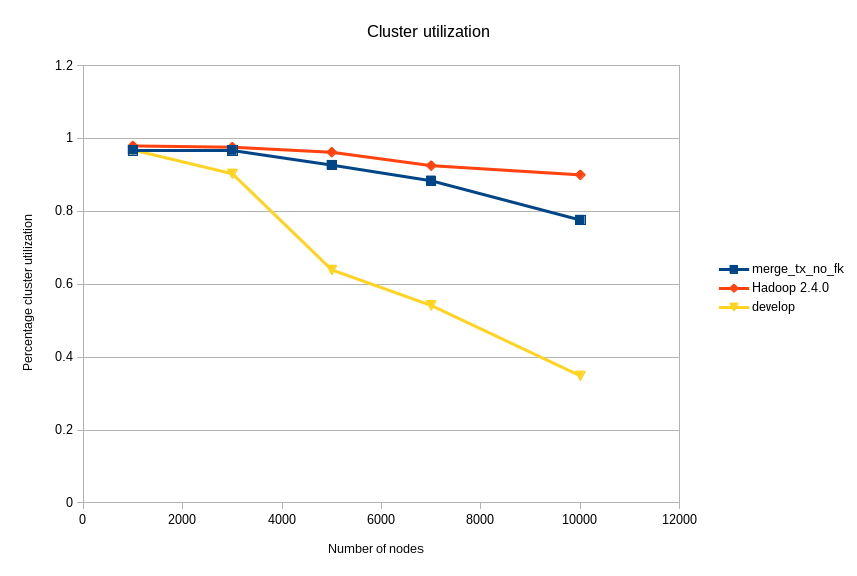
\includegraphics[scale=0.6]{resources/images/Evaluation/cluster_usage_final.png}
\caption{Cluster utilization comparison, Hops-YARN - Apache YARN}
\label{fig:ev_cluster_util_final}
\end{figure}

The second observation is the gap between \texttt{merge\_tx\_no\_fk} and
Hadoop 2.4.0 Until 7000 NodeManagers the difference is very small,
88$\%$ and 92$\%$ respectively. Even with the largest configuration
of 10000 nodes the difference is 13$\%$ in cluster utilization which
is not negligible but considering the lower recovery time of Hops-YARN
and the distributed ResourceManagers it might be a valid trade-off.

The next evaluation parameter for the project is the ratio of
heartbeats processed by the scheduler over the total number of
heartbeats. Hops-YARN has distributed the ResourceTrackerService which
receives heartbeats from NodeManagers, persists the information
received in NDB and then it is streamed to the master ResourceManager
which updates its view of the cluster. In Figure
\ref{fig:ev_hb_processed_final} is illustrated the heartbeat ratio for
the \texttt{develop} and \texttt{merge\_tx\_no\_fk} branch and Hadoop
2.4.0 We can observe a great improvement up until 4000
NodeManagers. Although the difference is small for the rest of the
simulations, it is constantly better than in \texttt{develop} branch
of Hops-YARN. Apache Hadoop never drops below 94$\%$ but it is
necessary to
mention that Apache YARN is a centralized architecture with no
communication latency between the ResourceTrackerService and the scheduler.

\begin{figure}
\centering
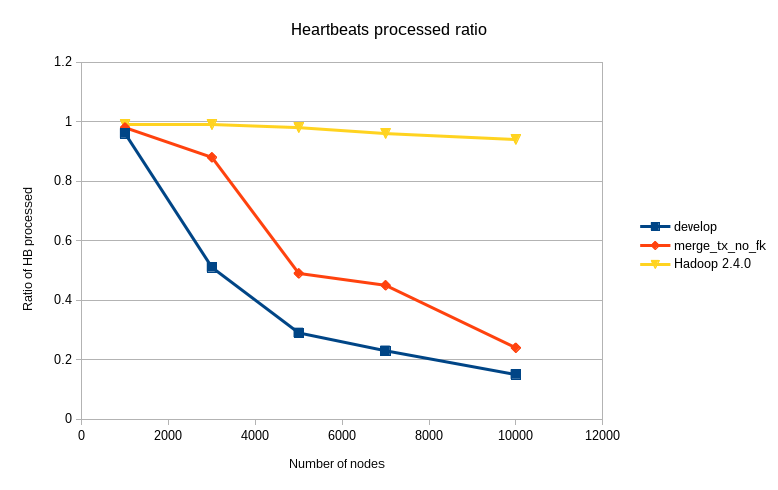
\includegraphics[scale=0.7]{resources/images/Evaluation/hb_processed_final.png}
\caption{Ratio of processed heartbeats}
\label{fig:ev_hb_processed_final}
\end{figure}

Finally, for the completeness of the evaluation it is worth to mention the
CPU utilization and memory
consumption (Figure  \ref{fig:ev_cpu_util_rm_rt}, \ref{fig:ev_mem_consumption_rm_rt}) of the
ResourceManager -- \textbf{bbc7} and the
ResourceTracker -- \textbf{bbc6}. Throughout the simulation with 10000 nodes in a
cluster, the average CPU usage of RM never went above 20$\%$ while for
the RT the maximum average is 45$\%$. Regarding the memory consumption
for the same simulation, both RM and RT never used more than 24GB of RAM.

\begin{figure}
\centering
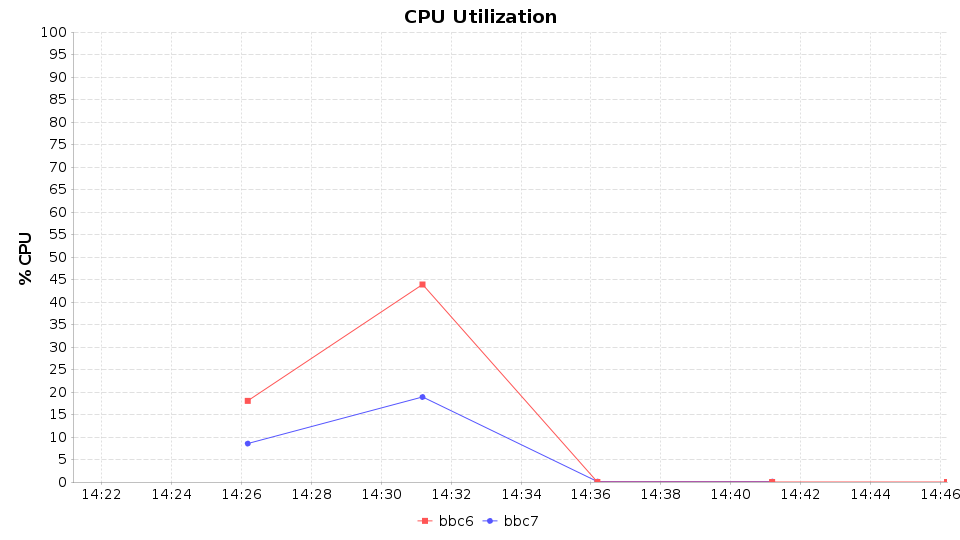
\includegraphics[scale=0.4]{resources/images/Evaluation/RM_RT_cpu_utilization.png}
\caption{CPU usage for RM (bbc7) and RT (bbc6)}
\label{fig:ev_cpu_util_rm_rt}
\end{figure}

\begin{figure}
\centering
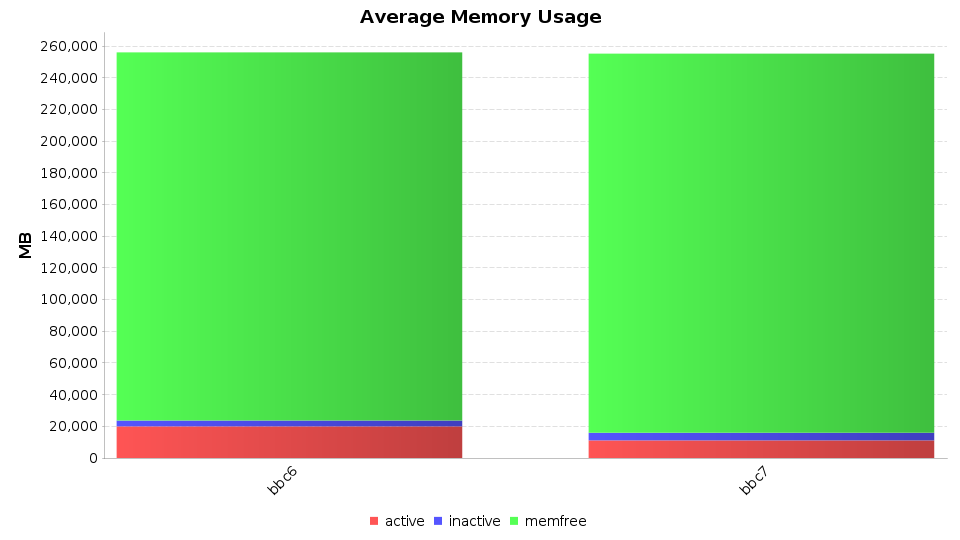
\includegraphics[scale=0.4]{resources/images/Evaluation/RM_RT_memory_usage.png}
\caption{Memory usage for RM (bbc7) and RT (bbc6)}
\label{fig:ev_mem_consumption_rm_rt}
\end{figure}
